\documentclass[a4 paper]{article}
\usepackage[inner=2.0cm,outer=2.0cm,top=2.5cm,bottom=2.5cm]{geometry}
\usepackage{setspace}
\usepackage[rgb]{xcolor}
\usepackage{verbatim}
\usepackage{subcaption}
\usepackage{amsgen,amsmath,amstext,amsbsy,amsopn,tikz,amssymb}
\usepackage{fancyhdr}
\usepackage[colorlinks=true, urlcolor=blue,  linkcolor=blue, citecolor=blue]{hyperref}
\usepackage[colorinlistoftodos]{todonotes}
\usepackage{rotating}
\usepackage{booktabs}
\newcommand{\ra}[1]{\renewcommand{\arraystretch}{#1}}

\newtheorem{thm}{Theorem}[section]
\newtheorem{prop}[thm]{Proposition}
\newtheorem{lem}[thm]{Lemma}
\newtheorem{cor}[thm]{Corollary}
\newtheorem{defn}[thm]{Definition}
\newtheorem{rem}[thm]{Remark}
\numberwithin{equation}{section}

\newcommand{\homework}[6]{
   \pagestyle{myheadings}
   \thispagestyle{plain}
   \newpage
   \setcounter{page}{1}
   \noindent
   \begin{center}
   \framebox{
      \vbox{\vspace{2mm}
    \hbox to 6.28in { {\bf CSE 211:~Discrete Mathematics \hfill {\small (#2)}} }
       \vspace{6mm}
       \hbox to 6.28in { {\Large \hfill #1  \hfill} }
       \vspace{6mm}
       \hbox to 6.28in { {\it Student: {\rm #3} \hfill  {\rm #5} \hfill  {\rm #6}} \hfill}
       \hbox to 6.28in { {\it Number: #4  \hfill #6}}
      \vspace{2mm}}
   }
   \end{center}
   \markboth{#5 -- #1}{#5 -- #1}
   \vspace*{4mm}
}

\newcommand{\problem}[2]{~\\\fbox{\textbf{Problem #1}}\hfill (#2 points)\newline\newline}
\newcommand{\subproblem}[1]{~\newline\textbf{(#1)}}
\newcommand{\D}{\mathcal{D}}
\newcommand{\Hy}{\mathcal{H}}
\newcommand{\VS}{\textrm{VS}}
\newcommand{\solution}{~\newline\textbf{\textit{(Solution)}} }

\newcommand{\bbF}{\mathbb{F}}
\newcommand{\bbX}{\mathbb{X}}
\newcommand{\bI}{\mathbf{I}}
\newcommand{\bX}{\mathbf{X}}
\newcommand{\bY}{\mathbf{Y}}
\newcommand{\bepsilon}{\boldsymbol{\epsilon}}
\newcommand{\balpha}{\boldsymbol{\alpha}}
\newcommand{\bbeta}{\boldsymbol{\beta}}
\newcommand{\0}{\mathbf{0}}


\begin{document}
\homework{Homework \#2}{Due: 07/12/20}{Yakup Talha Yolcu}{1801042609}{}{}


\problem{1: Relations}{15}
Draw the Hasse diagram for the “greater than or equal to” relation on $\{$0, 1, 2, 3, 4, 5$\}$.

\solution

Relation is :\newline
\{ (0,0) , (1,0) , (1,1) , (2,0) , (2,1) , (2,2) , (3,0) , (3,1) , (3,2) , (3,3) , (4,0) , (4,1) , (4,2) , (4,3) , (4,4) , (5,0) , (5,1) , (5,2) , (5,2) , (5,3) , (5,4) , (5,5) \}

Hasse diagram for ($\{$0, 1, 2, 3, 4, 5$\}$, $\leq$ ) is:

\begin{figure*}[htp]
	\centering
	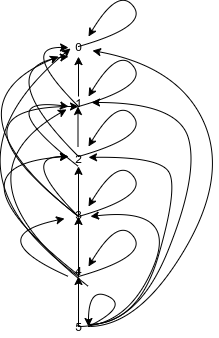
\includegraphics[scale=0.5]{diagram1.png}
	\caption{Original Graph}
	\label{fig: diagram}
	
\end{figure*}

Since we know that a poset MUST provide reflexivity, we also do not need the reflexive relations in A. Hence
A can be updated as:
A = \{ (1,0)  , (2,0) , (2,1) , (3,0) , (3,1) , (3,2) , (4,0) , (4,1) , (4,2) , (4,3)  , (5,0) , (5,1) , (5,2) , (5,2) , (5,3) , (5,4) \}
In the next step, remove the self-loops in Figure 2:

\begin{figure*}[htp]
	\centering
	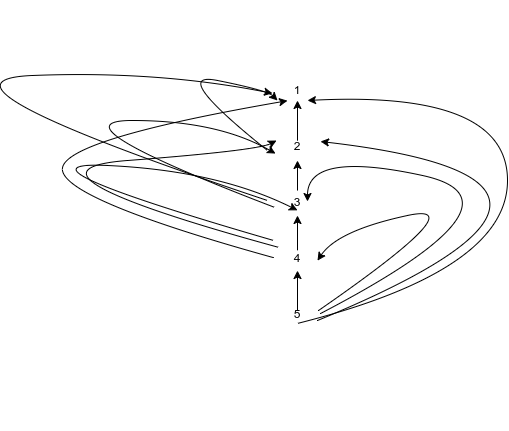
\includegraphics[scale=0.5]{a.png}
	\caption{The graph without self-loops}
	\label{fig: diagram}
	
\end{figure*}

\begin{figure*}[htp]
	\centering
	
\includegraphics[scale=0.5]{b.png}
	\caption{The hasse diagram of (\{ 0 , 1 , 2 , 3 , 4 , 5\}, \leq)}
	\label{fig: diagram}
	
\end{figure*}

Remove the transivite edges and the hasse diagram is obtained in Figure 3:


\newpage
\problem{2: Relations}{15}
Answer these questions for the poset ($\{\{$1$\}$, $\{$2$\}$, $\{$4$\}$, $\{$1, 2$\}$, $\{$1, 4$\}$, $\{$2, 4$\}$, $\{$3, 4$\}$, $\{$1, 3, 4$\}$, $\{$2, 3, 4$\}\}$, $\subseteq$).

Before the solution , we can draw a Hasse diagram for the POSET to determine maximal and minimal elements etc...\newline

\begin{figure*}[htp]
	\centering
	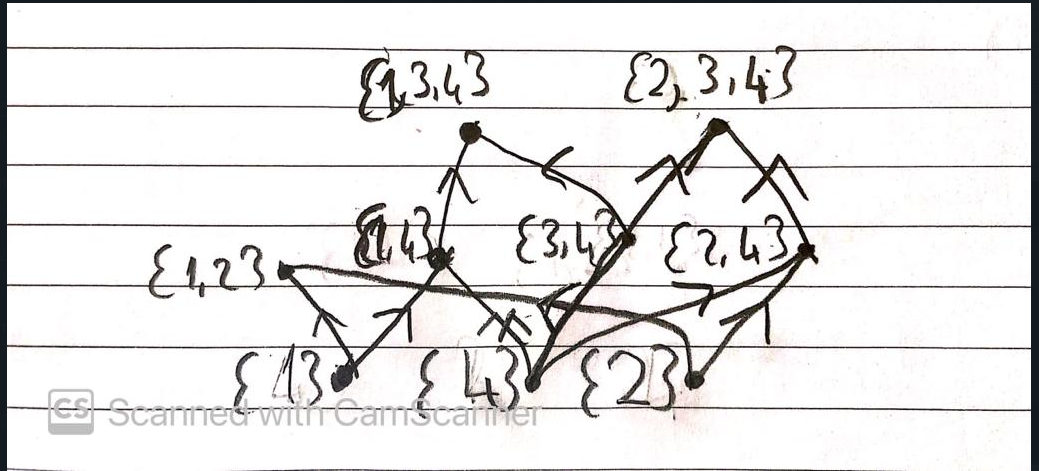
\includegraphics[scale=0.4]{diagram2.png}
	\caption{Hasse Diagram}
	\label{fig: diagram}
	
\end{figure*}

\subproblem{a} Find the maximal elements.
\solution
Maximal elements are : \{1,3,4\} and \{2,3,4\} They are at the top of the diagram.\newline
\subproblem{b} Find the minimal elements.
\solution
Minimal elements are : \{1\} , \{2\} and \{4\} They are at the bottom of the diagram.\newline
\subproblem{c} Is there a greatest element?
\solution
There is no greatest element because there is more than one maximal element.\newline
\subproblem{d} Find all upper bounds of $\{\{$2$\}$ , $\{$4$\}\}$.
\solution
Upper bounds of $\{\{$2$\}$ , $\{$4$\}\}$ are \{2,4\} and \{2,3,4\}.\newline
\subproblem{e} Find the least upper bound of $\{\{$2$\}$, $\{$4$\}\}$, if it exists.
\solution
Least upper bound of $\{\{$2$\}$, $\{$4$\}\}$ exists and its \{2,4\}.\newline
\subproblem{f} Find all lower bounds of $\{\{$1, 3, 4$\}$, $\{$2, 3, 4$\}\}$.
\solution
Lower bounds of \{$1, 3, 4$\} are : \{1\} , \{4\} , \{1,4\} and \{3,4\} \newline
Lower bounds of \{$2, 3, 4$\} are : \{2\} , \{4\} , \{3,4\} , \{2,4\} \newline
\subproblem{h} Find the greatest lower bound of $\{\{$1, 3, 4$\}$, $\{$2, 3, 4$\}\}$, if it exists.
\solution
Greatest lower bound of \{$1, 3, 4$\} does not exists.\newline
Greatest lower bound of \{$2, 3, 4$\} does not exists.\newline
\newpage


\problem{3: Relations}{70}
Remember that a relation $R$ on a set $A$ can have the properties reflexive, symmetric, anti-symmetric and transitive.

\begin{itemize}
	\item $\textbf{Reflexive: }$ R is reflexive if (a, a) $\in$ $R$, $\forall$ a $\in$ A.
	\item $\textbf{Symmetric: }$ R is symmetric if (b, a) $\in$ R whenever (a, b) $\in$ R, $\forall$ a, b $\in$ A.
	\item $\textbf{Anti-symmetric: }$ R is antisymmetric if $\forall$ a, b $\in$ A, (a, b) $\in$ R and (b, a) $\in$ R implies that a = b.
	\item $\textbf{Transitive: }$ R is transitive if $\forall$ a, b, c $\in$ A, (a, b) $\in$ R and (b, c) $\in$ R implies that (a, c) $\in$ R.
\end{itemize}

\end{document} 
